\documentclass[a4paper]{scrartcl}


\usepackage[utf8]{inputenc}
\usepackage[ngerman]{babel}
\usepackage{enumerate}
\usepackage{tikz}
\usepackage{fancyhdr}
\usepackage{lastpage}
\usepackage{verbatim}

\usepackage{listings}
\setlength{\parindent}{0mm}
\usepackage{graphicx}
\usepackage{amsmath}
\usepackage{algorithm2e}

\pagestyle{fancy}
\fancyhead[L]{SS 2017\\Joshua Hartmann}
\fancyhead[C]{Entwurf und Synthese von Eingebetteten Systemen\\Manfred Opel}
\fancyhead[R]{Blatt 7\\Nicolas Staller}

\fancyfoot[L]{}
\fancyfoot[C]{\thepage /\pageref{LastPage}}
\fancyfoot[R]{}

\renewcommand{\textheight}{700px}
\renewcommand{\footskip}{10px}
\newcommand*\xor{\mathbin{\oplus}}
\begin{document}	
	\section*{Aufgabe 1: Fragen zur Vorlesung}
	
	\begin{enumerate}[(a)]
		\item \hfill
		
		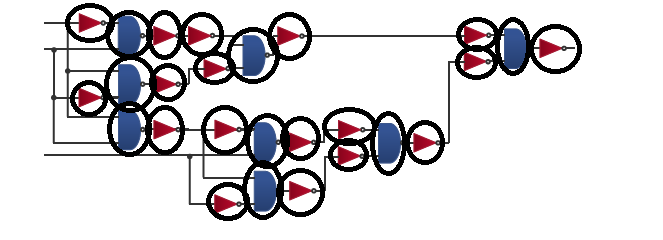
\includegraphics[scale=1]{1_subject_tree_max_cover}
		
		Es kann kein größeres Cover geben, da wir jeden einzelnen Baustein als eigenständige Gruppe betrachten. Jede aus diesen einzelnen Teilen zusammengesetzte Komponente hat eine kleiner Fläche als die Summe Einzelteile.
		
		Als Gesamtfläche erhält man:
		
		18 Inverter a 1 FE\\
		8 NAN2 a 2 FE\\
		
		also 18 + 2*8 = 32FE
		
		\item \hfill
		
		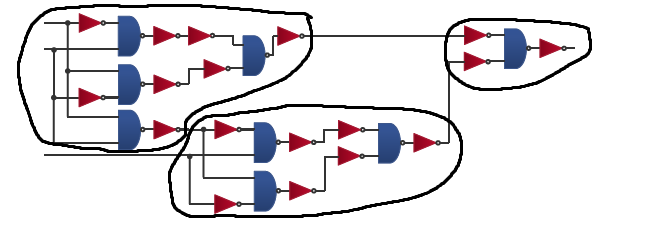
\includegraphics[scale=1]{1_subject_tree_12_cover}
		
		Teilt man den Subject Tree in je zwei Halbaddierer und ein NOR2 auf, so erhält man eine maximale Fläche von 12 FE.
		
	\end{enumerate}
	\newpage
	\section*{Aufgabe 2: RT-Synthese und Simulation einer 32-bit ALU}
	
	\begin{enumerate}[(a)]
		\item 
		\item 
		\item 
		\item Laut Area Report wird eine Fläche von 3248.924005 benötigt. Im Datasheet werden die einzelnen Komponenten mit Flächen in $um^2$ angegeben, daher nehmen wir an, dass auch die Gesamtfläche diese Einheit hat.
		
		\item Bei der Synthese wurde eine Taktperiode von 25ns angenommen. Die maximale Verzögerung in der Schaltung beträgt 4.21ns und laut Timing Report ergibt sich ein Slack von 20.75ns
		\item Der Result Ausgang ist mehrfach auf einem undefinierten Pegel, da das Signal wohl von mehreren Treibern beschrieben wird. Das liegt daran, dass unsere Taktperiode zu kurz gewählt wurde, weshalb eine Berechnung noch nicht fertig war, bevor eine andere bereits begonnen wurde.
		\item Taktperiode muss mindestens so lang sein wie die größte Verzögerung, die sich in der Timing Analyse ergeben hat.
	\end{enumerate}

	
\end{document}

